% ============================================================
%  DISCOVERY CURRICULUM — Journey 2, Module 3
%  "The Integral"
%  Compile with: pdflatex J2_M3.tex  (run twice for references)
% ============================================================

\documentclass[12pt, a4paper]{article}

\usepackage[a4paper, top=2.5cm, bottom=2.5cm, left=2.8cm, right=2.8cm, headheight=15pt]{geometry}
\usepackage{amsmath, amssymb, amsthm}
\usepackage{xcolor}
\usepackage{mdframed}
\usepackage{enumitem}
\usepackage{tikz}
\usetikzlibrary{arrows.meta, positioning, calc, patterns}
\usepackage{pgfplots}
\pgfplotsset{compat=1.18}
\usepackage{booktabs}
\usepackage{fancyhdr}
\usepackage{titlesec}
\usepackage{parskip}
\usepackage{hyperref}
\hypersetup{colorlinks=true, linkcolor=NavyBlue, urlcolor=NavyBlue}

% ── Colours ─────────────────────────────────────────────────
\definecolor{NavyBlue}{HTML}{1A3A5C}
\definecolor{MidBlue}{HTML}{2E6DA4}
\definecolor{Gold}{HTML}{C8922A}
\definecolor{LightBlue}{HTML}{EBF2FA}
\definecolor{LightGold}{HTML}{FDF4E3}
\definecolor{DarkGrey}{HTML}{3A3A3A}
\definecolor{BoxGreen}{HTML}{E8F5E9}
\definecolor{SidebarGrey}{HTML}{F5F5F5}

% ── Section formatting ───────────────────────────────────────
\titleformat{\section}{\Large\bfseries\color{NavyBlue}}{}{0em}{}[{\color{MidBlue}\vspace{2pt}\rule{\linewidth}{1.5pt}}]
\titleformat{\subsection}{\large\bfseries\color{MidBlue}}{}{0em}{}

% ── Header / Footer ─────────────────────────────────────────
\pagestyle{fancy}
\fancyhf{}
\fancyhead[L]{\small\color{DarkGrey}\textit{Discovery Curriculum}}
\fancyhead[R]{\small\color{DarkGrey}\textit{Journey 2 $\cdot$ Module 3}}
\fancyfoot[C]{\small\color{MidBlue}\thepage}
\renewcommand{\headrulewidth}{0.4pt}

% ── Environments ─────────────────────────────────────────────
\newmdenv[
  backgroundcolor=NavyBlue!7,
  linecolor=NavyBlue, linewidth=2pt,
  leftline=true, rightline=false, topline=false, bottomline=false,
  innerleftmargin=14pt, innerrightmargin=10pt,
  innertopmargin=10pt, innerbottommargin=10pt,
  skipabove=14pt, skipbelow=10pt
]{puzzlebox}

\newmdenv[
  backgroundcolor=LightGold,
  linecolor=Gold, linewidth=2pt,
  leftline=true, rightline=false, topline=false, bottomline=false,
  innerleftmargin=14pt, innerrightmargin=10pt,
  innertopmargin=10pt, innerbottommargin=10pt,
  skipabove=14pt, skipbelow=10pt
]{discoverybox}

\newmdenv[
  backgroundcolor=LightBlue,
  linecolor=MidBlue, linewidth=1.5pt,
  roundcorner=4pt,
  innerleftmargin=14pt, innerrightmargin=10pt,
  innertopmargin=10pt, innerbottommargin=10pt,
  skipabove=14pt, skipbelow=10pt
]{namebox}

\newmdenv[
  backgroundcolor=BoxGreen,
  linecolor=DarkGrey!35, linewidth=1pt,
  roundcorner=4pt,
  innerleftmargin=14pt, innerrightmargin=10pt,
  innertopmargin=10pt, innerbottommargin=10pt,
  skipabove=14pt, skipbelow=10pt
]{reflectionbox}

\newmdenv[
  backgroundcolor=SidebarGrey,
  linecolor=Gold, linewidth=1.2pt,
  leftline=true, rightline=false, topline=false, bottomline=false,
  innerleftmargin=12pt, innerrightmargin=10pt,
  innertopmargin=7pt, innerbottommargin=7pt,
  skipabove=10pt, skipbelow=10pt
]{thought}

\newcounter{problem}
\newenvironment{problem}[1][]{%
  \refstepcounter{problem}%
  \par\vspace{6pt}%
  \noindent\textbf{\color{MidBlue}Problem \theproblem}%
  \ifx&#1&\else\ \textit{(#1)}\fi\textbf{.}\enskip
}{\par\vspace{4pt}}

\newcounter{deepproblem}
\newenvironment{deepproblem}[1][]{%
  \refstepcounter{deepproblem}%
  \par\vspace{6pt}%
  \noindent\textbf{\color{NavyBlue}$\bigstar$\ Deep Problem \thedeepproblem}%
  \ifx&#1&\else\ \textit{(#1)}\fi\textbf{.}\enskip
}{\par\vspace{4pt}}

% ============================================================
\begin{document}
% ============================================================

\thispagestyle{empty}
\begin{center}
{\small\color{MidBlue}\textbf{DISCOVERY CURRICULUM}\quad$\cdot$\quad\textbf{JOURNEY 2: CHANGE}}

\vspace{0.6cm}
{\color{NavyBlue}\rule{\linewidth}{2pt}}
\vspace{0.5cm}

{\Huge\bfseries\color{NavyBlue}Module 3}\\[0.3cm]
{\LARGE\bfseries\color{MidBlue}The Integral}\\[0.4cm]
{\color{Gold}\rule{0.4\linewidth}{1.2pt}}\\[0.4cm]
{\large\itshape\color{DarkGrey}
The area under a curve and the reverse of the derivative\\[0.15cm]
are the same thing. This is not obvious. It is miraculous.}

\vspace{1cm}
\begin{tabular}{rl}
\color{DarkGrey}\textbf{Journey}           & Journey 2 --- Change \\[4pt]
\color{DarkGrey}\textbf{Module}            & 3 of 6 \\[4pt]
\color{DarkGrey}\textbf{Prerequisites}     & J2 Modules 1--2 (derivative, differentiation rules) \\[4pt]
\color{DarkGrey}\textbf{You will discover} & Riemann sums, definite integral, antiderivatives, Fundamental Theorem \\[4pt]
\color{DarkGrey}\textbf{Format}            & 8 problems $+$ 3 deep problems $\approx$ 14 pages \\
\end{tabular}

\vspace{1cm}
{\color{NavyBlue}\rule{\linewidth}{2pt}}
\end{center}

\vspace{0.5cm}

\noindent\textbf{Two separate problems.}
Journey~2 has so far been about rates of change: how fast does a function change at a point? Today we meet a completely different problem: how do you find the \emph{area} enclosed between a curve and the horizontal axis?

\medskip
These two questions --- \emph{rate of change} and \emph{area under a curve} --- look completely unrelated. One is about slopes. The other is about regions in the plane. The central discovery of this module is that they are, in a deep sense, the same question. This discovery is the Fundamental Theorem of Calculus, and it is arguably the most important theorem in all of mathematics.

\newpage

% ============================================================
\section{Part 1 \texorpdfstring{---}{--} The Puzzle}
% ============================================================

\begin{puzzlebox}
\textbf{The Opening Puzzle.}

A car's velocity (in m/s) is recorded every second:

\begin{center}
\begin{tabular}{ccccccc}
\toprule
$t$ (s) & 0 & 1 & 2 & 3 & 4 & 5 \\
\midrule
$v(t)$ (m/s) & 0 & 4 & 8 & 12 & 16 & 20 \\
\bottomrule
\end{tabular}
\end{center}

\textbf{Question 1.} Estimate how far the car travels in 5 seconds. How did you estimate? How accurate is your estimate?

\textbf{Question 2.} If $v(t) = 4t$, the exact distance is $\int_0^5 4t\,dt$. Before you know what this notation means: using the area interpretation, can you compute this geometrically? What shape is the region under the line $v = 4t$ from $t=0$ to $t=5$?

\textbf{Question 3.} Now suppose $v(t) = t^2$. The region under a parabola is not a simple geometric shape. How would you estimate the area? Could you make the estimate as accurate as you liked?
\end{puzzlebox}

% ============================================================
\section{Part 2 \texorpdfstring{---}{--} Exploration}
% ============================================================

\subsection{Step 1: Approximating area with rectangles}

\begin{problem}
\label{prob:riemann}
Consider $f(x) = x^2$ on $[0,1]$. We want to find the area under the curve.
\begin{enumerate}[label=(\alph*), topsep=2pt]
  \item Divide $[0,1]$ into 4 equal subintervals. For each, form a rectangle whose height is the function value at the \emph{left} endpoint. Draw these rectangles. Compute the total area (this is a \textbf{left Riemann sum}).
  \item Repeat using the \emph{right} endpoint of each subinterval (right Riemann sum).
  \item Repeat using the \emph{midpoint} of each subinterval (midpoint Riemann sum).
  \item Which estimate is an overestimate? Which is an underestimate? Why?
  \item Now repeat (a) and (b) with $n = 8$ subintervals. Are the estimates improving? What do you expect as $n \to \infty$?
\end{enumerate}
\end{problem}

\begin{center}
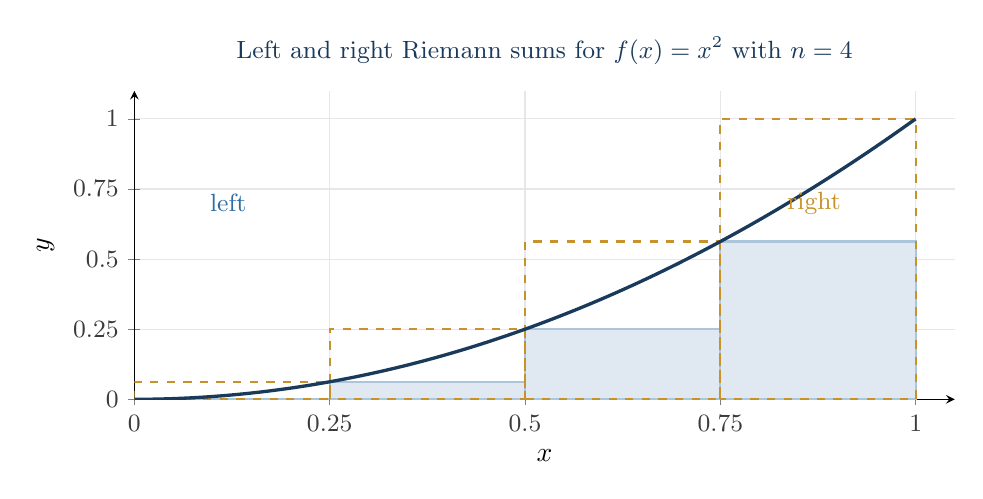
\begin{tikzpicture}
\begin{axis}[
  width=12cm, height=5.5cm,
  axis lines=left,
  xlabel={$x$}, ylabel={$y$},
  xmin=0, xmax=1.05, ymin=0, ymax=1.1,
  xtick={0,0.25,0.5,0.75,1},
  ytick={0,0.25,0.5,0.75,1},
  tick label style={font=\small, color=DarkGrey},
  grid=major, grid style={DarkGrey!12},
  title={\small\color{NavyBlue}Left and right Riemann sums for $f(x)=x^2$ with $n=4$},
]
% Left sum rectangles (dashed blue)
\foreach \x/\h in {0/0, 0.25/0.0625, 0.5/0.25, 0.75/0.5625} {
  \addplot[MidBlue!40, fill=MidBlue!15, thick] coordinates {(\x,0)(\x,\h)(\x+0.25,\h)(\x+0.25,0)(\x,0)};
}
% Right sum rectangles (solid gold, outline only)
\foreach \x/\h in {0/0.0625, 0.25/0.25, 0.5/0.5625, 0.75/1.0} {
  \addplot[Gold, thick, dashed] coordinates {(\x,0)(\x,\h)(\x+0.25,\h)(\x+0.25,0)(\x,0)};
}
% Curve
\addplot[NavyBlue, very thick, domain=0:1, samples=100] {x^2};
\node[font=\small, color=MidBlue] at (axis cs: 0.12, 0.7) {left};
\node[font=\small, color=Gold] at (axis cs: 0.87, 0.7) {right};
\end{axis}
\end{tikzpicture}
\end{center}

\begin{problem}
\label{prob:riemann_limit}
For $f(x) = x^2$ on $[0,1]$ with $n$ equal subintervals using right endpoints:
\begin{enumerate}[label=(\alph*), topsep=2pt]
  \item The $k$-th right endpoint is $x_k = k/n$. Write the right Riemann sum $R_n = \sum_{k=1}^{n} f(x_k) \cdot \frac{1}{n}$.
  \item Substitute $f(x_k) = (k/n)^2$ to get $R_n = \frac{1}{n^3}\sum_{k=1}^{n} k^2$.
  \item Use the formula $\sum_{k=1}^{n} k^2 = \frac{n(n+1)(2n+1)}{6}$ to find a closed form for $R_n$.
  \item Take $\lim_{n\to\infty} R_n$. What is the area under $x^2$ from 0 to 1?
  \item Repeat for $f(x) = x^3$ using $\sum_{k=1}^n k^3 = \left(\frac{n(n+1)}{2}\right)^2$. Do you notice a pattern?
\end{enumerate}
\end{problem}

\begin{thought}
\textbf{Archimedes and the method of exhaustion.}
The idea of approximating curved areas by sums of rectangles is ancient. Archimedes (287--212 BCE) computed the area of a parabolic segment using his ``method of exhaustion'' --- filling the region with triangles of decreasing size and summing an infinite geometric series. He obtained the correct answer, $\frac{4}{3}$ times the triangle with the same base and height, nearly 2000 years before calculus. What Archimedes lacked was not the idea but the general machinery: he had to devise a clever new geometric argument for each curve. Newton and Leibniz provided the general method that works for \emph{all} curves at once.
\end{thought}

\subsection{Step 2: The definite integral as a limit}

\begin{problem}
\label{prob:integral_defn}
Let $f$ be a continuous function on $[a,b]$. Divide $[a,b]$ into $n$ equal subintervals of width $\Delta x = (b-a)/n$. Choose any point $x_k^*$ in the $k$-th subinterval.
\begin{enumerate}[label=(\alph*), topsep=2pt]
  \item Write the general Riemann sum $S_n = \sum_{k=1}^{n} f(x_k^*)\,\Delta x$.
  \item Explain geometrically: each term $f(x_k^*)\,\Delta x$ is the area of a thin rectangle. For $f$ taking negative values, what does a negative term represent?
  \item The definite integral $\int_a^b f(x)\,dx$ is defined as $\lim_{n\to\infty} S_n$ when this limit exists and is the same for all choices of $x_k^*$. What does the integral represent when $f$ takes both positive and negative values?
  \item Use the Riemann sum definition to verify $\int_0^1 c\,dx = c$ for a constant $c$ (the area of a rectangle).
  \item Use it to verify $\int_0^b x\,dx = b^2/2$ (the area of a triangle). Sketch.
\end{enumerate}
\end{problem}

\subsection{Step 3: The antiderivative}

\begin{problem}
\label{prob:antideriv}
A function $F$ is called an \textbf{antiderivative} of $f$ if $F'(x) = f(x)$.
\begin{enumerate}[label=(\alph*), topsep=2pt]
  \item Find an antiderivative of $f(x) = 2x$. Is it unique?
  \item If $F$ and $G$ are both antiderivatives of $f$, what can you say about $F - G$? Prove it. (Hint: what function has derivative 0 everywhere?)
  \item Find antiderivatives of: $x^3$, $\cos x$, $e^x$, $\frac{1}{x}$, $x^n$ for $n \neq -1$.
  \item Why does $x^n$ require $n \neq -1$ in part (c)? What is the antiderivative of $\frac{1}{x}$?
  \item We write $\int f(x)\,dx = F(x) + C$ (the \textbf{indefinite integral}). Explain the $+C$ and why it cannot be dropped.
\end{enumerate}
\end{problem}

\subsection{Step 4: The Fundamental Theorem}

You now have two separate objects: the definite integral (area under a curve, computed as a limit of Riemann sums) and the antiderivative (a function whose derivative is $f$). They look completely different. The next problem reveals they are secretly the same.

\begin{problem}
\label{prob:ftc_discover}
Define the \textbf{accumulation function} $A(x) = \int_a^x f(t)\,dt$, the area under $f$ from $a$ to $x$.
\begin{enumerate}[label=(\alph*), topsep=2pt]
  \item Let $f(t) = 2t$ and $a = 0$. Compute $A(x) = \int_0^x 2t\,dt$ geometrically (the area is a triangle). What function do you get?
  \item Differentiate your answer for $A(x)$. What do you get? Does it surprise you?
  \item Now compute $A(x+h) - A(x)$ geometrically. This is the area of a thin strip above the interval $[x, x+h]$. Approximate this area by a rectangle of height $f(x)$ and width $h$. Compute $\frac{A(x+h)-A(x)}{h}$ and take $h\to 0$.
  \item You have just sketched a proof that $A'(x) = f(x)$. State this as a theorem.
  \item Use this theorem to evaluate $\int_0^1 x^2\,dx$. Compare with your Riemann sum calculation from Problem~\ref{prob:riemann_limit}.
\end{enumerate}
\end{problem}

\begin{center}
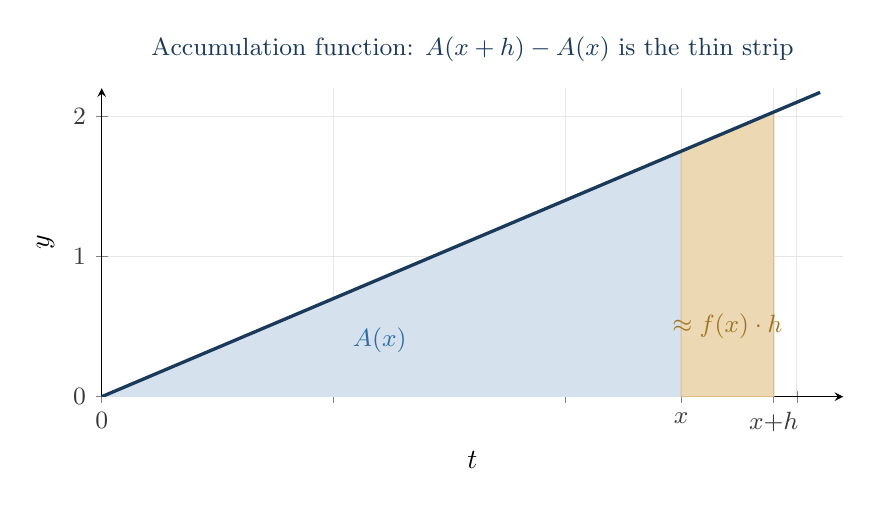
\begin{tikzpicture}
\begin{axis}[
  width=11cm, height=5.5cm,
  axis lines=left,
  xlabel={$t$}, ylabel={$y$},
  xmin=0, xmax=3.2, ymin=0, ymax=2.2,
  xtick={0,1,2,2.5,2.9,3},
  xticklabels={$0$,$\,$,$\,$,$x$,$x{+}h$,$\,$},
  ytick={0,1,2},
  tick label style={font=\small, color=DarkGrey},
  grid=major, grid style={DarkGrey!12},
  title={\small\color{NavyBlue}Accumulation function: $A(x+h)-A(x)$ is the thin strip},
]
% Shaded area A(x)
\addplot[MidBlue!20, fill=MidBlue!15] coordinates {(0,0)(0,0)(2.5,0)};
\addplot[MidBlue!20, fill=MidBlue!20, domain=0:2.5, samples=50] {0.7*x} \closedcycle;
% Thin strip A(x+h)-A(x)
\addplot[Gold!60, fill=Gold!35, domain=2.5:2.9, samples=10] {0.7*x} \closedcycle;
% Curve
\addplot[NavyBlue, very thick, domain=0:3.1, samples=80] {0.7*x};
% Labels
\node[font=\small, color=MidBlue] at (axis cs:1.2, 0.4) {$A(x)$};
\node[font=\small, color=Gold!80!black] at (axis cs:2.7, 0.5) {$\approx f(x)\cdot h$};
\draw[<->, Gold, thick] (axis cs:2.5,-0.15) -- (axis cs:2.9,-0.15) node[midway,below,font=\tiny]{$h$};
\end{axis}
\end{tikzpicture}
\end{center}

\begin{problem}
\label{prob:ftc_apply}
The Fundamental Theorem gives $\int_a^b f(x)\,dx = F(b) - F(a)$ where $F' = f$.
\begin{enumerate}[label=(\alph*), topsep=2pt]
  \item Evaluate $\int_0^3 x^2\,dx$, $\int_1^4 \sqrt{x}\,dx$, $\int_0^{\pi} \sin x\,dx$, $\int_1^e \frac{1}{x}\,dx$.
  \item Evaluate $\int_0^{2\pi} \sin x\,dx$. The integrand is not always positive. Explain the answer geometrically.
  \item Find a function $f$ such that $\int_1^x f(t)\,dt = x^3 - x^2 + 2$ for all $x$. (Differentiate both sides.)
  \item A car accelerates from rest with $a(t) = 6t\,\text{m/s}^2$. Find its velocity $v(t)$ and position $s(t)$, given $v(0) = 0$ and $s(0) = 0$.
  \item The net area $\int_a^b f\,dx$ can be zero even if $f \neq 0$. The total area is $\int_a^b |f|\,dx$. For $f(x) = \sin x$ on $[0, 2\pi]$: compute both net area and total area.
\end{enumerate}
\end{problem}

\begin{thought}
\textbf{Why the Fundamental Theorem is miraculous.}
Area and slope seem to have nothing to do with each other. One is a two-dimensional quantity (region in a plane); the other is a one-dimensional quantity (steepness of a line). The Fundamental Theorem says they are inverse operations. Computing the area under $f$ from $a$ to $x$ gives a function whose derivative is $f$. This is as surprising as saying: if you count the total rainfall from the beginning of the year up to each day, the rate at which that total is increasing is today's rainfall. Which is, of course, obvious stated that way. The miracle is that ``obvious'' statement, stated in full generality, is a deep theorem.
\end{thought}

\begin{problem}
\label{prob:integral_techniques}
Each integral requires a technique beyond direct application of the FTC.
\begin{enumerate}[label=(\alph*), topsep=2pt]
  \item \textbf{Substitution} (reverse chain rule): evaluate $\int 2x(x^2+1)^5\,dx$. Let $u = x^2+1$.
  \item Evaluate $\int_0^1 xe^{x^2}\,dx$ using substitution.
  \item \textbf{Integration by parts} (reverse product rule): the rule is $\int u\,dv = uv - \int v\,du$. Evaluate $\int x e^x\,dx$ by choosing $u = x$, $dv = e^x\,dx$.
  \item Evaluate $\int x \ln x\,dx$ by parts.
  \item Evaluate $\int \ln x\,dx$ by parts, using the trick $\ln x = \ln x \cdot 1$.
\end{enumerate}
\end{problem}

% ============================================================
\section{Part 3 \texorpdfstring{---}{--} Discovery}
% ============================================================

\begin{discoverybox}
\textbf{What have we built?}

\textbf{First.} The definite integral $\int_a^b f(x)\,dx$ is the signed area under the curve, defined as a limit of Riemann sums. It is a number.

\textbf{Second.} The antiderivative (indefinite integral) $\int f(x)\,dx = F(x) + C$ is a family of functions, defined by $F' = f$.

\textbf{Third.} The Fundamental Theorem connects them:
\[
  \frac{d}{dx}\int_a^x f(t)\,dt = f(x) \qquad \text{and} \qquad \int_a^b f(x)\,dx = F(b) - F(a).
\]
The first part says: differentiate an integral, get back the integrand. The second says: integrate by finding an antiderivative and evaluating at the endpoints. These two statements are not the same, but together they are the entire practical content of calculus.

\medskip
\textbf{The deeper question.} Differentiation has a clean algebraic structure: product rule, chain rule, derivations. Does integration? What is the ``chain rule'' for integrals? (There is one: substitution. What is its algebraic structure?)
\end{discoverybox}

% ============================================================
\section{Part 4 \texorpdfstring{---}{--} Naming the Ideas}
% ============================================================

\begin{namebox}
\textbf{The definite integral and the Fundamental Theorem.}

The \textbf{definite integral} of $f$ on $[a,b]$ is
\[
  \int_a^b f(x)\,dx \;=\; \lim_{n\to\infty}\sum_{k=1}^n f(x_k^*)\,\Delta x.
\]

A function $F$ is an \textbf{antiderivative} of $f$ if $F' = f$. Any two antiderivatives differ by a constant.

\medskip
\textbf{Fundamental Theorem of Calculus, Part I.} If $f$ is continuous on $[a,b]$:
\[
  \frac{d}{dx}\int_a^x f(t)\,dt \;=\; f(x).
\]

\textbf{Fundamental Theorem of Calculus, Part II.} If $F' = f$:
\[
  \int_a^b f(x)\,dx \;=\; F(b) - F(a).
\]

\textbf{Integration by substitution} (reverse chain rule): $\displaystyle\int f(g(x))g'(x)\,dx = \int f(u)\,du$, where $u = g(x)$.

\textbf{Integration by parts} (reverse product rule): $\displaystyle\int u\,dv = uv - \int v\,du$.
\end{namebox}

% ============================================================
\section{Part 5 \texorpdfstring{---}{--} Deep Problems}
% ============================================================

\begin{deepproblem}[Proving the Fundamental Theorem rigorously]
\begin{enumerate}[label=(\alph*)]
  \item Let $f$ be continuous on $[a,b]$ and $A(x) = \int_a^x f(t)\,dt$. Write the difference quotient $\frac{A(x+h)-A(x)}{h} = \frac{1}{h}\int_x^{x+h} f(t)\,dt$.
  \item The \textbf{Mean Value Theorem for Integrals} states that there exists $c \in [x, x+h]$ such that $\int_x^{x+h} f(t)\,dt = f(c)\cdot h$. Accept this for now and complete the proof that $A'(x) = f(x)$.
  \item Now prove Part II: if $F' = f$ and $A(x) = \int_a^x f(t)\,dt$, then $A' = F' = f$, so $A - F$ is constant. Evaluate at $x = a$ to find the constant. Conclude $\int_a^b f(x)\,dx = F(b) - F(a)$.
  \item Why does the proof require $f$ to be continuous? What can go wrong if $f$ has a jump discontinuity?
  \item \textit{(Hard.)} The function $f(x) = \begin{cases}1 & x \geq 0 \\ 0 & x < 0\end{cases}$ has a jump at $x=0$. Show that $A(x) = \int_{-1}^x f(t)\,dt$ is continuous at $x=0$ but not differentiable there. Reconcile this with Part I of the FTC.
\end{enumerate}
\end{deepproblem}

\begin{deepproblem}[Improper integrals]
The integral $\int_a^\infty f(x)\,dx$ is defined as $\lim_{R\to\infty}\int_a^R f(x)\,dx$ when this limit exists.
\begin{enumerate}[label=(\alph*)]
  \item Evaluate $\int_1^\infty \frac{1}{x^2}\,dx$. Does it converge?
  \item Evaluate $\int_1^\infty \frac{1}{x}\,dx$. Does it converge? Reconcile with the divergence of the harmonic series $\sum 1/n$.
  \item For which values of $p$ does $\int_1^\infty \frac{1}{x^p}\,dx$ converge? Find the value in terms of $p$.
  \item The Gaussian integral $\int_{-\infty}^{\infty} e^{-x^2}\,dx = \sqrt{\pi}$ (from Module~5, Journey~1). Accept this result. Use it to find $\int_{-\infty}^{\infty} e^{-x^2/2}\,dx$.
  \item The \textbf{Gamma function} extends the factorial to non-integers: $\Gamma(n) = \int_0^\infty t^{n-1}e^{-t}\,dt$. Use integration by parts to show $\Gamma(n+1) = n\,\Gamma(n)$. Compute $\Gamma(1)$ and deduce $\Gamma(n) = (n-1)!$ for positive integers $n$.
\end{enumerate}
\end{deepproblem}

\begin{deepproblem}[Computing areas and volumes]
\begin{enumerate}[label=(\alph*)]
  \item Find the area enclosed between $y = x^2$ and $y = x$ by integrating the difference $x - x^2$ between the intersection points.
  \item A solid of revolution is formed by rotating $y = \sqrt{x}$ for $x\in[0,4]$ around the $x$-axis. The cross-section at position $x$ is a circle of radius $\sqrt{x}$. Set up and evaluate the integral $\int_0^4 \pi(\sqrt{x})^2\,dx$ for its volume.
  \item The \textbf{arc length} of a curve $y = f(x)$ from $a$ to $b$ is $\int_a^b \sqrt{1 + [f'(x)]^2}\,dx$. Derive this formula by approximating the curve by small straight segments.
  \item Find the arc length of $y = x^{3/2}$ from $x = 0$ to $x = 4$.
  \item \textit{(Hard.)} The \textbf{surface area} of the solid of revolution from (b) is $\int_0^4 2\pi f(x)\sqrt{1+[f'(x)]^2}\,dx$. Evaluate it. Why does this formula involve the arc length element $\sqrt{1+[f'(x)]^2}$?
\end{enumerate}
\end{deepproblem}

% ============================================================
\section{Part 6 \texorpdfstring{---}{--} Reflection}
% ============================================================

\begin{reflectionbox}
\textbf{Your reflection task.}

\begin{enumerate}
  \item \textbf{On the miracle.} Write the Fundamental Theorem in your own words --- not the formula, but what it says. Then explain why it is surprising. Is there an analogy in a completely different domain where two apparently unrelated operations turn out to be inverses of each other?

  \item \textbf{On Archimedes.} Archimedes computed the area of a parabolic segment in 250 BCE without calculus. He had the right answer but the wrong method, in the sense that he could not generalise it. Is a method that gives the right answer for the wrong reasons a good method? What does ``understanding'' a result mean, beyond being able to produce it?

  \item \textbf{On the $+C$.} Every antiderivative carries an arbitrary constant $+C$. In physics, this constant usually has physical meaning (initial position, initial velocity). Write down a physical situation where the value of $C$ is determined by an initial condition, and one where two different values of $C$ give two qualitatively different physical behaviours.

  \item \textbf{Looking ahead.} Module~4 asks what happens when integration is applied to rates of change in several variables simultaneously --- the first step toward differential equations. You have solved $\frac{dP}{dt} = kP$ (exponential growth). What would you do with $\frac{dP}{dt} = kP(1-P/K)$ (logistic growth)? Can you separate variables?
\end{enumerate}
\end{reflectionbox}

\medskip
\noindent\textbf{Looking ahead.}
Module~4 studies the behaviour of functions: where do they increase, decrease, have maxima and minima? The derivative tells us all of this, and the integral lets us compute areas, lengths, and volumes. Together they are the complete toolkit of single-variable calculus. Module~5 then moves to ordinary differential equations --- the language in which physics is written. And Module~6 opens the door to multivariable calculus, where all of this generalises to higher dimensions.

\vspace{1.4cm}
\begin{center}
{\color{MidBlue}\rule{0.5\linewidth}{0.8pt}}\\[6pt]
{\small\color{DarkGrey}\textit{End of Journey 2, Module 3 --- The Integral}}\\[4pt]
{\small\color{DarkGrey}Continue to: \textbf{Module 4 --- Applications: Shape, Optimisation, and Motion}}\\[6pt]
{\color{MidBlue}\rule{0.5\linewidth}{0.8pt}}
\end{center}

\end{document}